\documentclass{beamer}

\usepackage[utf8]{inputenc}
\usepackage[romanian]{babel}
\usepackage{hyperref}
\usepackage{graphicx}

% Tema prezentării
\usetheme{Madrid}
\usecolortheme{default}

\title[Analiză și Testare Tax Calculator]{Analiza și Testarea Aplicației Tax Calculator}
\subtitle{Proiect TSS 2026}
\author{Stefan Tacu}
\date{\today}

\begin{document}

% 1. Slide de titlu
\begin{frame}
    \titlepage
\end{frame}

% 2. Introducere și Configurație
\begin{frame}{1. Introducere și Configurație}
    \begin{itemize}
        \item \textbf{Obiectiv:} Testarea riguroasă a unei aplicații de calcul fiscal.
        \item \textbf{Stack Tehnic:}
        \begin{itemize}
            \item Python 3.13.2, Pytest 8.1.1
            \item Radon (Complexity), Mutmut (Mutation)
            \item Coverage.py (Structural Coverage)
        \end{itemize}
        \item \textbf{Funcționalitate:} Calcul taxe pe categorii (Salary, Business, Crypto, etc.) cu aplicare de deduceri complexe.
    \end{itemize}
\end{frame}

% 3. Testare Funcțională (Black-Box)
\begin{frame}{2. Testare Funcțională (Black-Box)}
    \begin{itemize}
        \item \textbf{Tehnici:} Equivalence Partitioning \& Boundary Value Analysis.
        \item \textbf{Clase de Echivalență:}
        \begin{itemize}
            \item Venit: Valid [0, 1M], Invalid (<0, >1M).
            \item Vârstă: Valid [0, 150], Invalid.
            \item Categorii: 6 categorii valide + ramură default.
        \end{itemize}
        \item \textbf{Status:} 100\% teste funcționale trecute.
    \end{itemize}
\end{frame}

% 4. Analiza Structurală: Teoria McCabe
\begin{frame}{3. Analiza Structurală: Teoria McCabe}
    \begin{itemize}
        \item \textbf{Complexitate Ciclomatică (CC):} Măsură a numărului de circuite liniar independente.
        \item \textbf{Formula McCabe:} $V(G) = e - n + 2p$ (unde $p=1$ pentru o subrutină).
        \item \textbf{Aplicație:} În proiectul nostru, $V(G) = 41$ (Grad F).
        \item \textbf{Testarea Circuitelor Independente:}
        \begin{itemize}
            \item Identifică limita superioară pentru numărul de căi necesare acoperirii ramurilor.
            \item \textbf{Set de bază:} Orice cale prin program se poate forma ca o combinație din acest set.
        \end{itemize}
        \item \textbf{Avantaj:} Setul poate fi generat pentru a garanta \textit{Branch Coverage} 100\%.
    \end{itemize}
\end{frame}

% 5. Rezultate Acoperire Structurală
\begin{frame}{4. Rezultate Acoperire Structurală}
    \begin{center}
        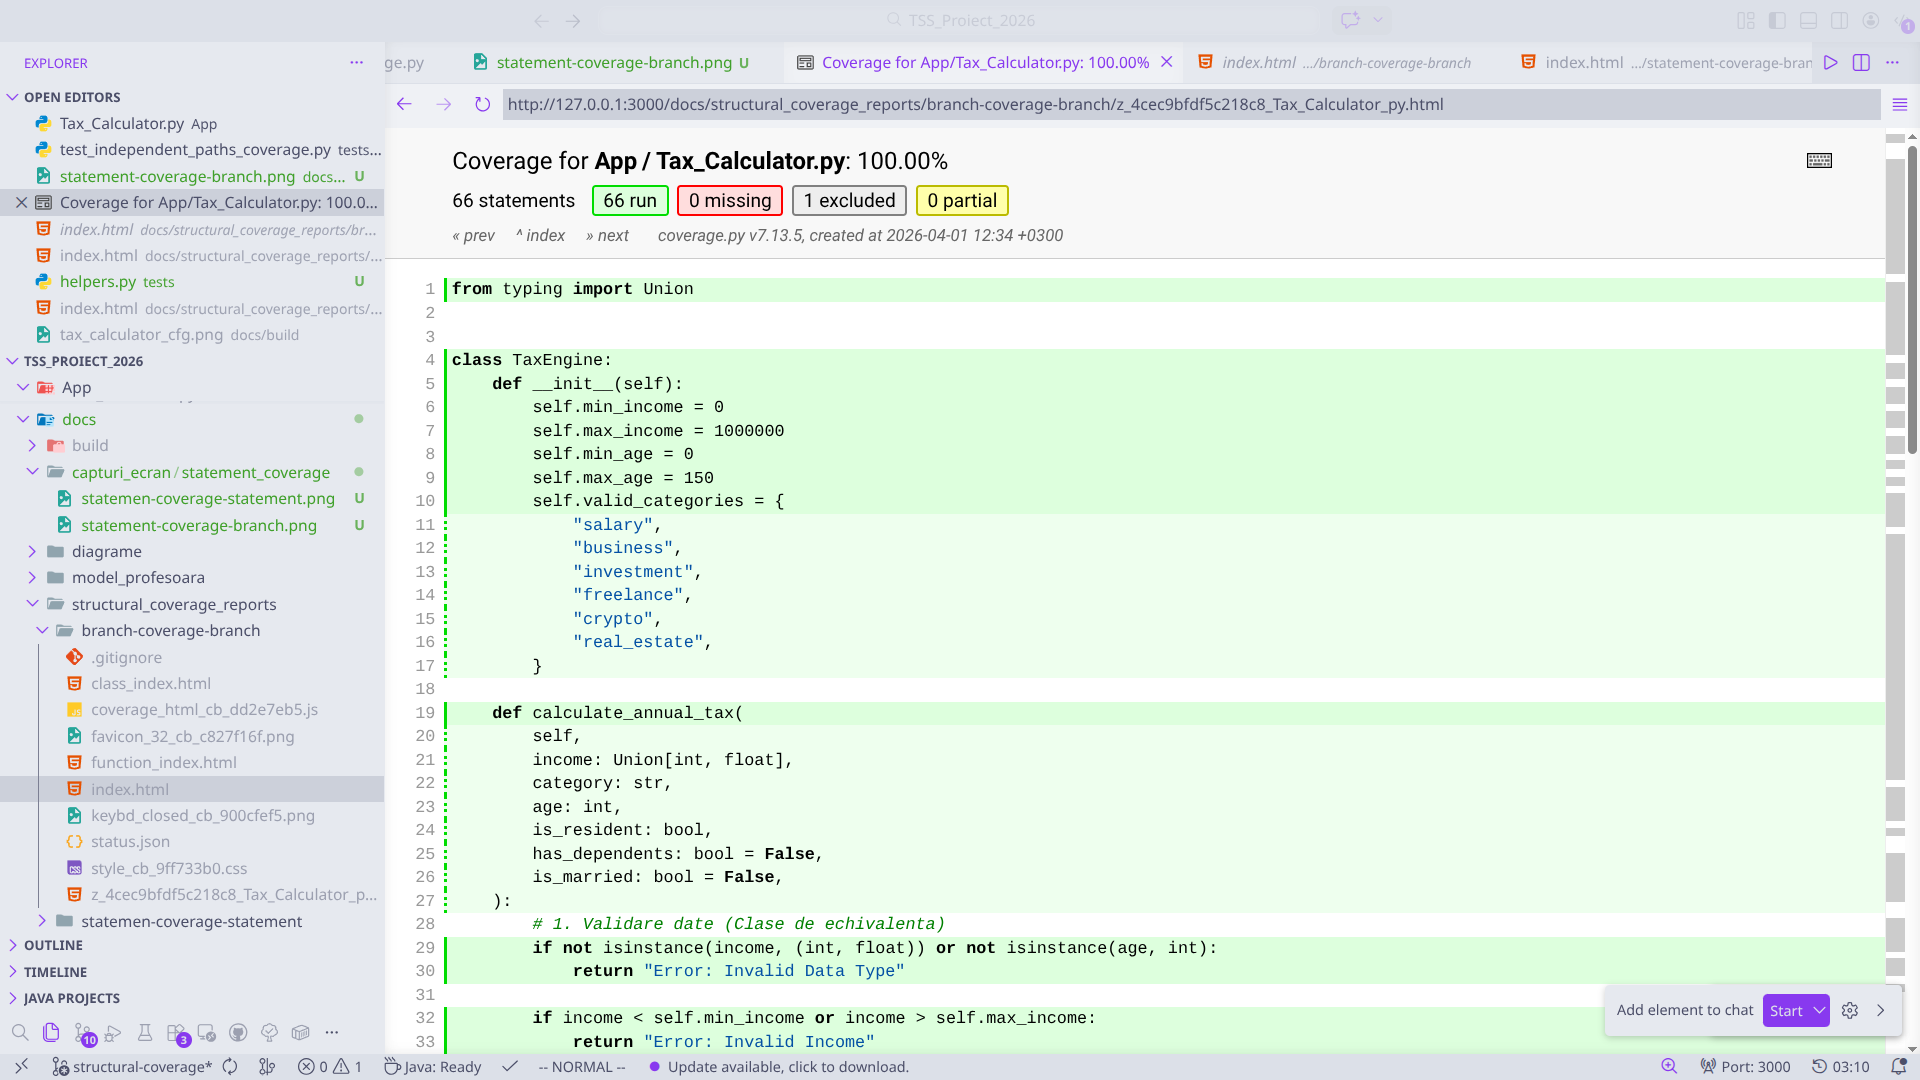
\includegraphics[width=0.85\textwidth]{capturi_ecran/statement_coverage/branch-coverage-branch.png}
    \end{center}
    \begin{itemize}
        \item \textbf{Statement Coverage:} 100\%
        \item \textbf{Branch Coverage:} 100\% (obținut după rafinarea suitei de teste pentru a acoperi ramurile \texttt{else} implicite).
    \end{itemize}
\end{frame}

% 6. Testarea prin Mutație (Mutation Testing)
\begin{frame}{5. Testarea prin Mutație (Mutation Testing)}
    \begin{itemize}
        \item \textbf{Instrument:} \texttt{mutmut} (mutanți de ordin 1).
        \item \textbf{Rezultate Automate:}
        \begin{itemize}
            \item Total mutanți: 228
            \item Omorâți: 181
            \item \textbf{Mutation Score: 79.3\%}
        \end{itemize}
        \item \textbf{Analiză Manuală:} Scor de 72.7\% pe un eșantion reprezentativ de 22 de mutanți.
    \end{itemize}
\end{frame}

% 7. Analiza Mutanților: Supraviețuitori
\begin{frame}{6. Analiza Mutanților: Supraviețuitori}
    \begin{itemize}
        \item \textbf{Mutanți Echivalenți:} Modificarea \texttt{>} în \texttt{>=} la praguri unde diferența este zero (ex: Business category).
        \item \textbf{Lipsă Precizie:} Supraviețuirea la modificarea rotunjirii (\texttt{round(tax, 1)}) a indicat aserțiuni prea permisive.
        \item \textbf{Îmbunătățire:} Rezultatele au condus la adăugarea de teste de frontieră mai stricte pentru categoriile Investment și Freelance.
    \end{itemize}
\end{frame}

% 8. Utilizare AI: GitHub Copilot
\begin{frame}{7. Utilizare AI: GitHub Copilot}
    \begin{itemize}
        \item \textbf{Eficiență:} Creștere cu ~40\% a vitezei de scriere a testelor de tip boiler-plate.
        \item \textbf{Puncte Forte:} Sugestii rapide pentru clasele de echivalență standard.
        \item \textbf{Puncte Slabe:} Riscul de "halucinații" la calcule matematice complexe și omiterea cazurilor de frontieră pe logica de CC 41.
        \item \textbf{Concluzie:} AI-ul este un copilot, dar decizia de testare rămâne la inginer.
    \end{itemize}
\end{frame}

% 9. Concluzii
\begin{frame}{8. Concluzii}
    \begin{itemize}
        \item \textbf{Rigoare:} Branch Coverage de 100\% este necesar dar nu suficient fără Mutation Testing.
        \item \textbf{Complexitate:} Codul cu CC 41 (Rank F) este greu de întreținut și necesită teste automate dense.
        \item \textbf{Validare:} Integrarea metodelor manuale cu cele automate oferă cel mai înalt grad de încredere în software.
    \end{itemize}
\end{frame}

% 10. Final
\begin{frame}
    \centering
    \Huge \textbf{Vă mulțumesc!} \\
    \bigskip
    \Large Întrebări și discuții.
\end{frame}

\end{document}
